\documentclass[12pt]{article}

\usepackage{import}
\usepackage{standalone}

\usepackage[top=4cm, right=2cm, bottom=2.7cm, left=2cm]{geometry}

\usepackage{wrapfig}
\usepackage{tabulary}
\usepackage{float}
\usepackage{pifont}
\usepackage{background}
\usepackage{tikz}


\pagestyle{empty}
\setlength{\parindent}{0pt}

\begin{document}
	\begin{minipage}{\textwidth}
		\section{De Magische Koffer \hfill\small Bron: Bebras}
			
			Ward de bever vaart met zijn boot op een meer met enkele eilanden. Zijn doel is om tot aan de vlag te varen.
			
			Ward kan de automatische piloot van zijn boot programmeren met een reeks opdrachten die de boot van punt naar punt op de kaart zullen verplaatsen. Elke opdracht geeft een verplaatsing aan van een aantal stappen in één van de acht mogelijke richtingen. Bijvoorbeeld, de opdracht \textbf{2NW} verplaatst de boot 2 stappen naar het noordwesten.
			
			\begin{figure}[H]
				\begin{minipage}{0.7\linewidth}
					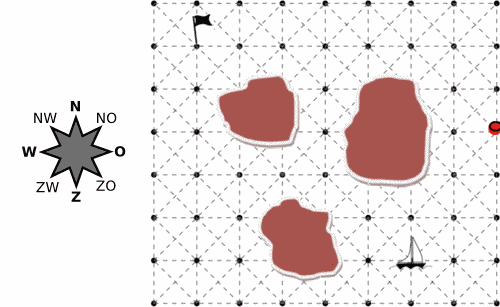
\includegraphics[width=\linewidth]{image1}
				\end{minipage}
				\hfill
				\begin{minipage}{0.25\linewidth}
					\centering
					Het programma \textbf{1N, 2NO} bijvoorbeeld, stuurt de boot
					naar de boei in 3 stappen.
					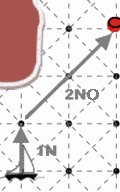
\includegraphics[width=0.9\linewidth]{image2}
				\end{minipage}
			\end{figure}
	
			Welke van de volgende programma's laat de boot toe om de eilanden te vermijden en de vlag te bereiken in het \textbf{minimum aantal stappen}?
	
			\begin{table}[H]
				\centering
				\begin{tabular}{|c l|}
					\hline
					\textbf{A} &  2NW, 2W, 1N, 1W, 2N \\ 
					\textbf{B} &  2NW, 3N, 3W \\
					\textbf{C} &  2NW, 2Wm 1NW, 2N \\ 
					\textbf{D} &  5NW \\ 
					\hline
				\end{tabular}
			\end{table}
	\end{minipage} \\ \\
	
\end{document}	